\subhead{Reading the lower bound in the public records}
The metallic lower bound resolves the gap and both edge penalties jointly. For a metal with common edge $t$, the vertical distance above the curve below equals the formation-energy penalty up to rounding.
\[
 B(t)=7.84+[ (5.73-t)/0.5 ]_+^2+[(t-4.50)/0.5]_+^2 .
\]
Moving the common edge to the left alleviates the CBM violation while increasing the VBM violation. Moving it to the right has the opposite effect. Their thresholds are separated by 1.23 eV. Figure~\ref{fig:regimes} shows why neither edge adjustment can compensate for zero gap.

\begin{figure}[htbp]
\centering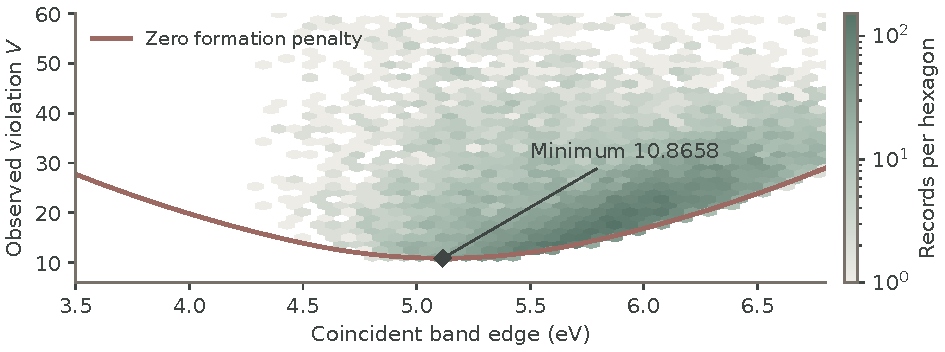
\includegraphics[width=\linewidth]{figures/physical_regimes.pdf}
\caption{Zero-gap records in files 02 and 03, grouped into hexagons in the displayed window. The color scale counts records. The curve gives the lower bound $B(t)$ and the diamond marks its minimum at $t=5.115$ eV.}\label{fig:regimes}
\end{figure}

Positive gap narrows the public screen from 15,225 records to 573 and retains all 110 with $V<1$. Even with the true gap known, only $110/573=19.2\%$ of the gapped records pass this relaxed test. In O3, 28 of 132 gapped compositions have $V<1$. In NO2, the ratio is 14 of 70, and in N3 none of 18 passes. These counts are descriptive. In particular, the hidden set was constructed to contain the exact targets, which changes the interpretation of any full-population prevalence estimate.
